%	Preamble. Put stuff here to define global settings.
% SJK: Document template originally from Andy Maloney "untitled.tex"
\documentclass{article}

%	Packages used.
\usepackage{amsmath}
\usepackage{fullpage}
\usepackage{graphicx}
\usepackage{caption}
\usepackage{subcaption}
%% see: http://en.wikibooks.org/wiki/LaTeX/Floats,_Figures_and_Captions#Subfloats
%	Define new commands for fun and expediated typing.
\newcommand{\bdm}{\begin{displaymath}}
\newcommand{\edm}{\end{displaymath}}

\begin{document}
	Quick summary of connectivity-constrained clustering (2.2.4.1.2.1. Ward clustering).

	\begin{itemize}
		\item I replicated the code with Lena, plot\_lena\_ward\_segmentation.py
		\item I also tried it out with a picture I took of nachos.  I used imagemagic and gimp to make the image smaller and grayscale.  I really didn't learn much from this exercise, since I don't have a real purpose yet.
		\item  don't know why I get fewer than 15 or 5 segments when looking at the nachos image. I also don't know how to include color. At this point I'll ignore and move on.
	\end{itemize}

    \begin{figure}
            \centering
            \begin{subfigure}[b]{0.3\textwidth}
                    \centering
                    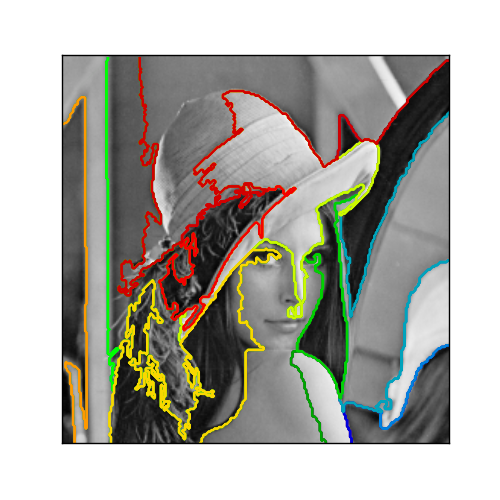
\includegraphics[width=\textwidth]{lena_ward_15.png}
                    \caption{Lena Ward clustering segmentation, 15 clusters}
                    \label{fig:lena15}
            \end{subfigure}%
            ~ %add desired spacing between images, e. g. ~, \quad, \qquad etc.
              %(or a blank line to force the subfigure onto a new line)
            \begin{subfigure}[b]{0.3\textwidth}
                    \centering
                    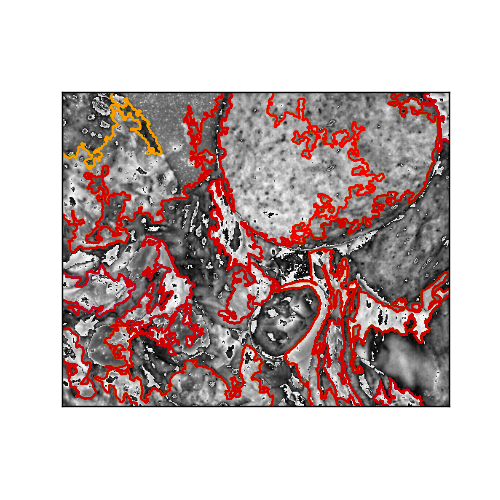
\includegraphics[width=\textwidth]{nachosgray_crop_ward_15.png}
                    \caption{Nachos, 15 clusters}
                    \label{fig:nachos15}
            \end{subfigure}
            ~ %add desired spacing between images, e. g. ~, \quad, \qquad etc.
              %(or a blank line to force the subfigure onto a new line)
            \begin{subfigure}[b]{0.3\textwidth}
                    \centering
                    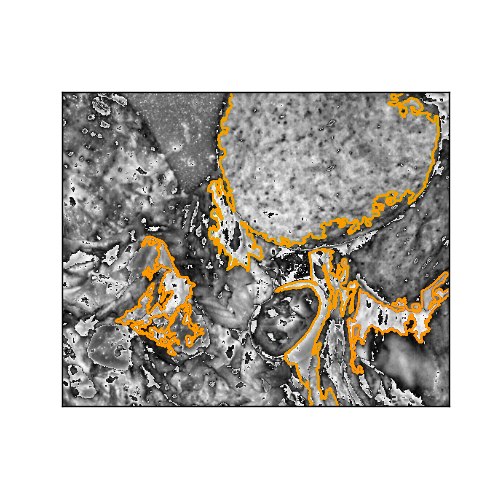
\includegraphics[width=\textwidth]{nachosgray_crop_ward_5.png}
                    \caption{nachos 5 clusters}
                    \label{fig:nachos5}
            \end{subfigure}
            \caption{Image segmentation by Ward clustering}\label{fig:images3}
    \end{figure}


\end{document}
